% !TeX spellcheck = de_DE
\section{Multiskalenanalyse}
%
Das mathematische Äquivalent der Beschreibung eines Objektes mithilfe von Koeffizienten ist ein Vektorraum. Jedes Element des Vektorraums kann dabei bei gegebener (Schauder-)Basis als eine endliche bzw. abzählbar unendliche Folge von Koeffizienten dargestellt werden. Wir wollen uns hier, den später präsentierten Anwendungen entsprechend, auf endlich-dimensionale Vektorräume beschränken.

\subsection{Mathematische Konstruktion}
Es bezeichne $\Phi^N=\{\phi^N_1, ..., \phi^N_{\dim V_N}\}$ die zu den gespeicherten Koeffizienten gehörige Basis und $V_N:=\mathrm{span}(\Phi^N)$ den zugehörigen Vektorraum.\\
Für die Multiskalenanalyse wird nun ein Set von geschachtelten Vektorräumen\begin{equation*}
V_0\subset V_1\subset V_2\subset ...\subset V_{N-1}\subset V_N
\end{equation*}mit zugehörigen Basen\begin{equation*}
\Phi^i=\{\phi^i_1, ..., \phi^i_{\dim V_i}\}
\end{equation*}benötigt. Die Wahl eines Skalarproduktes über $V_N$ fixiert dann die orthogonalen Komplemente der $V_i$:\begin{equation*}
W_i:=V_i^\perp \mathrm{\ \ in\ \ } V_{i+1}\qquad\Leftrightarrow\qquad W_i\oplus V_i=V_{i+1}
\end{equation*}Die induzierte Norm übernimmt dabei die Rolle eines Fehlermaßes, dies sollte bei der Wahl des Skalarproduktes bedacht werden.
Nun müssen noch die Basisvektoren der orthogonalen Komplemente gewählt werden:\begin{equation*}
\Psi^i=\{\psi^i_1, ..., \psi^i_{\dim W_i}\}
\end{equation*}Die $\phi^i_j$s werden als Skalenfunktionen, die $\psi^i_j$s als Wavelets (von englisch wave: Welle und französisch -lette: klein) bezeichnet.\\
Standardmäßig werden Funktionen des $\mathcal{L}^2([0,1])$ unter dem Standardskalarprodukt\begin{equation*}
\left\langle f\mid g\right\rangle :=\int_{0}^{1}f(x)\cdot g(x)\mathrm{d}x
\end{equation*}betrachtet. Um eine gleichmäßige Informationsdichte zu ermöglichen werden die Skalenfunktionen dann ihrem Namen entsprechend als skalierte und verschobene Versionen der $V_0$-Basisvektoren gewählt:\begin{equation*}
\phi^i_{k\cdot j}(x)=\begin{cases}
\phi^0_j(m^i x-(k-1)),&m^i x-(k-1)\in[0,1]\\
0, &\mathrm{sonst}
\end{cases};\qquad 1\leq k\leq m^i, \ \ m\in \mathbb{N}.
\end{equation*}Der Skalierungsfaktor $m$ legt dabei die Vektorraumdimensionen fest:\begin{equation*}
\dim V_i=m^i\cdot \dim V_0;\qquad\dim W_i=(m-1)m^i\cdot \dim V_0
\end{equation*}Auch die Wavelets können dann als skalierte und verschobene Versionen der $\{\Psi^0\}$ gewählt werden. Es ist meist erstrebenswert, dass sie eine Orthonormalbasis der $W_i$ bilden, einen kleinen Träger besitzen und bis zu einem gewissen Maße stetig differenzierbar sind. Wavelets welche alle drei Eigenschaften erfüllen sind als Daubechies-Wavelets bekannt.

\subsection{Die Filter Bank}
Die Konstruktion der orthogonalen Komplemente $W_i$ erlaubt es nun die Elemente jedes Vektorraums $V_i=V_{i-1}\oplus W_{i-1}$ in der Basis $\{\phi^{i-1}_1, ..., \phi^{i-1}_{\dim V_{i-1}}, \psi^{i-1}_1, ..., \psi^{i-1}_{\dim W_{i-1}}\}$ darzustellen. Die Basistransformationsmatrix $T^i_{sf\rightarrow wl}$ ist mit der Wahl der Basisvektoren eindeutig festgelegt durch\begin{equation*}
\left[ \Phi^i\right] =\left[ \Phi^{i-1}\mid \Psi^{i-1}\right] \cdot T^i_{sf\rightarrow wl}=:\left[ \Phi^{i-1}\mid \Psi^{i-1}\right]\left[ \frac{\ A^i\ }{\ B^i\ }\right].
\end{equation*}Die Matrizen $A^i$ und $B^i$ sind einzeln betrachtet Projektionen, welche $V_i$ auf die Unterräume $V_{i-1}$ bzw. $W_{i-1}$ abbilden. Sie werden als Analyse-Filter bezeichnet. Die Rücktransformation ist gegeben durch\begin{equation*}
T^i_{wl\rightarrow sf}=\left[ \frac{\ A^i\ }{\ B^i\ }\right]^{-1}=:\left[ P^i\mid Q^i\right].
\end{equation*}Die Matrizen $P^i$ und $Q^i$ werden dabei als Synthese Filter bezeichnet.\\
Ist nun ein Koeffizientenvektor $C^i$ zur Basis $\Phi^i$ gegeben, so erhalten wir die Koeffizienten $C^{i-1}$ des Unterraums zur Basis $\Phi^{i-1}$ und die Detailkoeffizienten $D^i$ zur Wavelet-Basis $\Psi^i$ durch\begin{equation*}
	\begin{cases}
	&A^i\cdot C^i=C^{i-1}\\
	&B^i\cdot C^i=D^{i-1}.
	\end{cases}
\end{equation*}
Um die Elemente des $V_N$ in der Basis des $V_0\oplus W_0 \oplus...\oplus W_{N-1}$ also komplett mithilfe der Wavelets darzustellen, werden nun die Analyse Filter rekursiv angewendet. Dieser Prozess wird Filter Bank genannt.
\begin{figure}[h]
	\centering
	\includegraphics[page=11, trim=60 695 305 100, clip, width=0.7\textwidth]{4_wavelet_final[14255].pdf}
	\caption{Die Filter Bank}
\end{figure}\\
Werden nun in dieser Wavelet-Basis Koeffizienten weggelassen, erhalten wir nicht mehr ein unvollständiges Bild (bzw. Vektorraumelement), sondern ein niedriger aufgelöstes Bild (bzw. Element eines skalierten Unterraums). Wir wollen nun zur Anschauung ein einfaches und doch für die Kompression sehr praktikables (siehe Kap. 5) Beispiel einführen: die Haar-Wavelets.


\section{Haar-Wavelets}

Die Haar-Skalenfunktionen und -Wavelets sind nur stückweise stetige Funktionen auf $\mathcal{L}^2([0,1])$ bzw. $\mathcal{L}^2([0,1])\times\mathcal{L}^2([0,1])$. Dafür bilden sie eine Orthonormalbasis, besitzen einen kleinen Träger und sind insgesamt sehr einfach zu handhaben. Die Skalenfunktionen entsprechen dabei den einzelnen Pixeln eines Bildes, während die Wavelets die Differenz benachbarter Pixel darstellen. Die zweidimensionale Variante ist somit für eine beispielhafte Anwendung der Bildkompression hervorragend geeignet. Zunächst sollen jedoch die eindimensionalen Haar-Wavelets eingeführt werden, um die Konstruktion ihres zweidimensionalen Äquivalents zu erleichtern.

\subsection{1D Haar-Wavelets}
Die 1D Haar-Wavelets sind im Funktionenraum $\mathcal{L}^2([0,1])$ unter dem Standardskalarprodukt definiert.
Es ist ausreichend die zu skalierende Skalenfunktion $\phi^0$ und das zugehörige Wavelet $\psi^0$ anzugeben:\begin{align*}
	\phi^0(x) &= \chi_{[0,1)}(x)\\
	\psi^0(x) &= \chi_{[0,\frac{1}{2})}(x)-\chi_{[\frac{1}{2}, 1)}(x)
\end{align*}
Alle weiteren Skalenfunktionen und Wavelets werden durch die folgende Skalierung und Verschiebung erzeugt:\begin{align*}
	\phi^i_{k}(x)&=\begin{cases}
	\sqrt{2^i}\phi^0(2^i x-k)),&2^i x-k\in[0,1]\\
	0, &\mathrm{sonst}
	\end{cases};\qquad 0\leq k\leq 2^i-1\\
	\psi^i_{k}(x)&=\begin{cases}
	\sqrt{2^i}\psi^0(2^i x-k)),&2^i x-k\in[0,1]\\
	0, &\mathrm{sonst}
	\end{cases};\qquad 0\leq k\leq 2^i-1
\end{align*}Damit sind auch die geschachtelten Vektorräume $V^i_{1D}$, die orthogonalen Komplemente $W^i_{1D}$ und die Analyse und Synthese Filter $A^i$, $B^i$, $P^i$ sowie $Q^i$ festgelegt und auch leicht zu bestimmen.
\begin{figure}[h]
	\centering
	\includegraphics[page=3, trim=166 490 346 276, clip, width=0.3\textwidth]{4_wavelet_final[14255].pdf}
	\includegraphics[page=3, trim=141 187 365 570, clip, width=0.3\textwidth]{4_wavelet_final[14255].pdf}
	\caption{Skalenfunktionen (links) und Wavelet-Basis (rechts) des $V_{1D}^3$}
\end{figure}

\subsection{2D Haar-Wavelets}
Die 2D Haar-Wavelets sind im Funktionenraum $\mathcal{L}^2([0,1])\times\mathcal{L}^2([0,1])$ unter folgendem Skalarprodukt definiert:\begin{equation*}
	\left\langle f, g\right\rangle _{2D}:=\int_{0}^{1}\int_{0}^{1}f(x,y)g(x,y)\mathrm{d}x\mathrm{d}y
\end{equation*}
Die geschachtelten Vektorräume sowie Skalenfunktionen werden als kartesisches Produkt zweier eindimensionaler Haar-Räume bzw. Skalenfunktionen gesetzt:\begin{align*}
	V^i_{2D}&:= V^i_{1D}\times V^i_{1D}\\
	\Phi^i_{2D}(x, y)&:=\{\phi^i_k(x)\phi^i_l(y)\mid \phi^i_k, \phi^i_l\in\Phi^i_{1D} \}
\end{align*}
Für die Konstruktion der Wavelets gibt es zwei gängige Varianten:
\paragraph{Standard-Konstruktion}~\\
Hierbei wird die 1D Wavelet-Basis $\Phi_{1D}^0\cup\Psi_{1D}^0\cup...\cup\Psi_{1D}^{i}$ für x- und y-Achse separat angewandt:\begin{align*}
	\Psi^i_{2D}(x, y)&:=\{\psi^i_k(x)\lambda^i_l(y)\mid \psi^i_k\in\Psi_{1D}^{i};\lambda^i_l\in\Phi_{1D}^0\cup\Psi_{1D}^0\cup...\cup\Psi_{1D}^{i} \}\\
	&\cup\ \{\lambda^i_k(x)\psi^i_l(y)\mid \psi^i_l\in\Psi_{1D}^{i};\lambda^i_k\in\Phi_{1D}^0\cup\Psi_{1D}^0\cup...\cup\Psi_{1D}^{i} \}
\end{align*}Bildlich gesprochen wird die 1D Wavelet-Transformation zuerst auf die Zeilen angewendet, um dann die erhaltenen transformierten Koeffizienten spaltenweise einer zweiten 1D Wavelet-Transformation zu unterziehen.
\paragraph{Nicht-Standard-Konstruktion}~\\
Bei der Nicht-Standard-Konstruktion werden als Ausgangspunkt die Wavelets $\Psi^0_{2D}$ der Standard-Konstruktion verwendet und in x- und y-Richtung gleichzeitig skaliert:\begin{equation*}
	\tilde\Psi^i_{2D}(x, y):=\{2^i\psi^0(2^ix-k, 2^iy-l)\mid \psi^0 \in \Psi^0_{2D}\}
\end{equation*}Bildlich werden ebenfalls nacheinander 1D Wavelet-Transformationen auf Zeilen und Spalten angewendet, allerdings abwechselnd.
\begin{figure}[h]
	\centering
	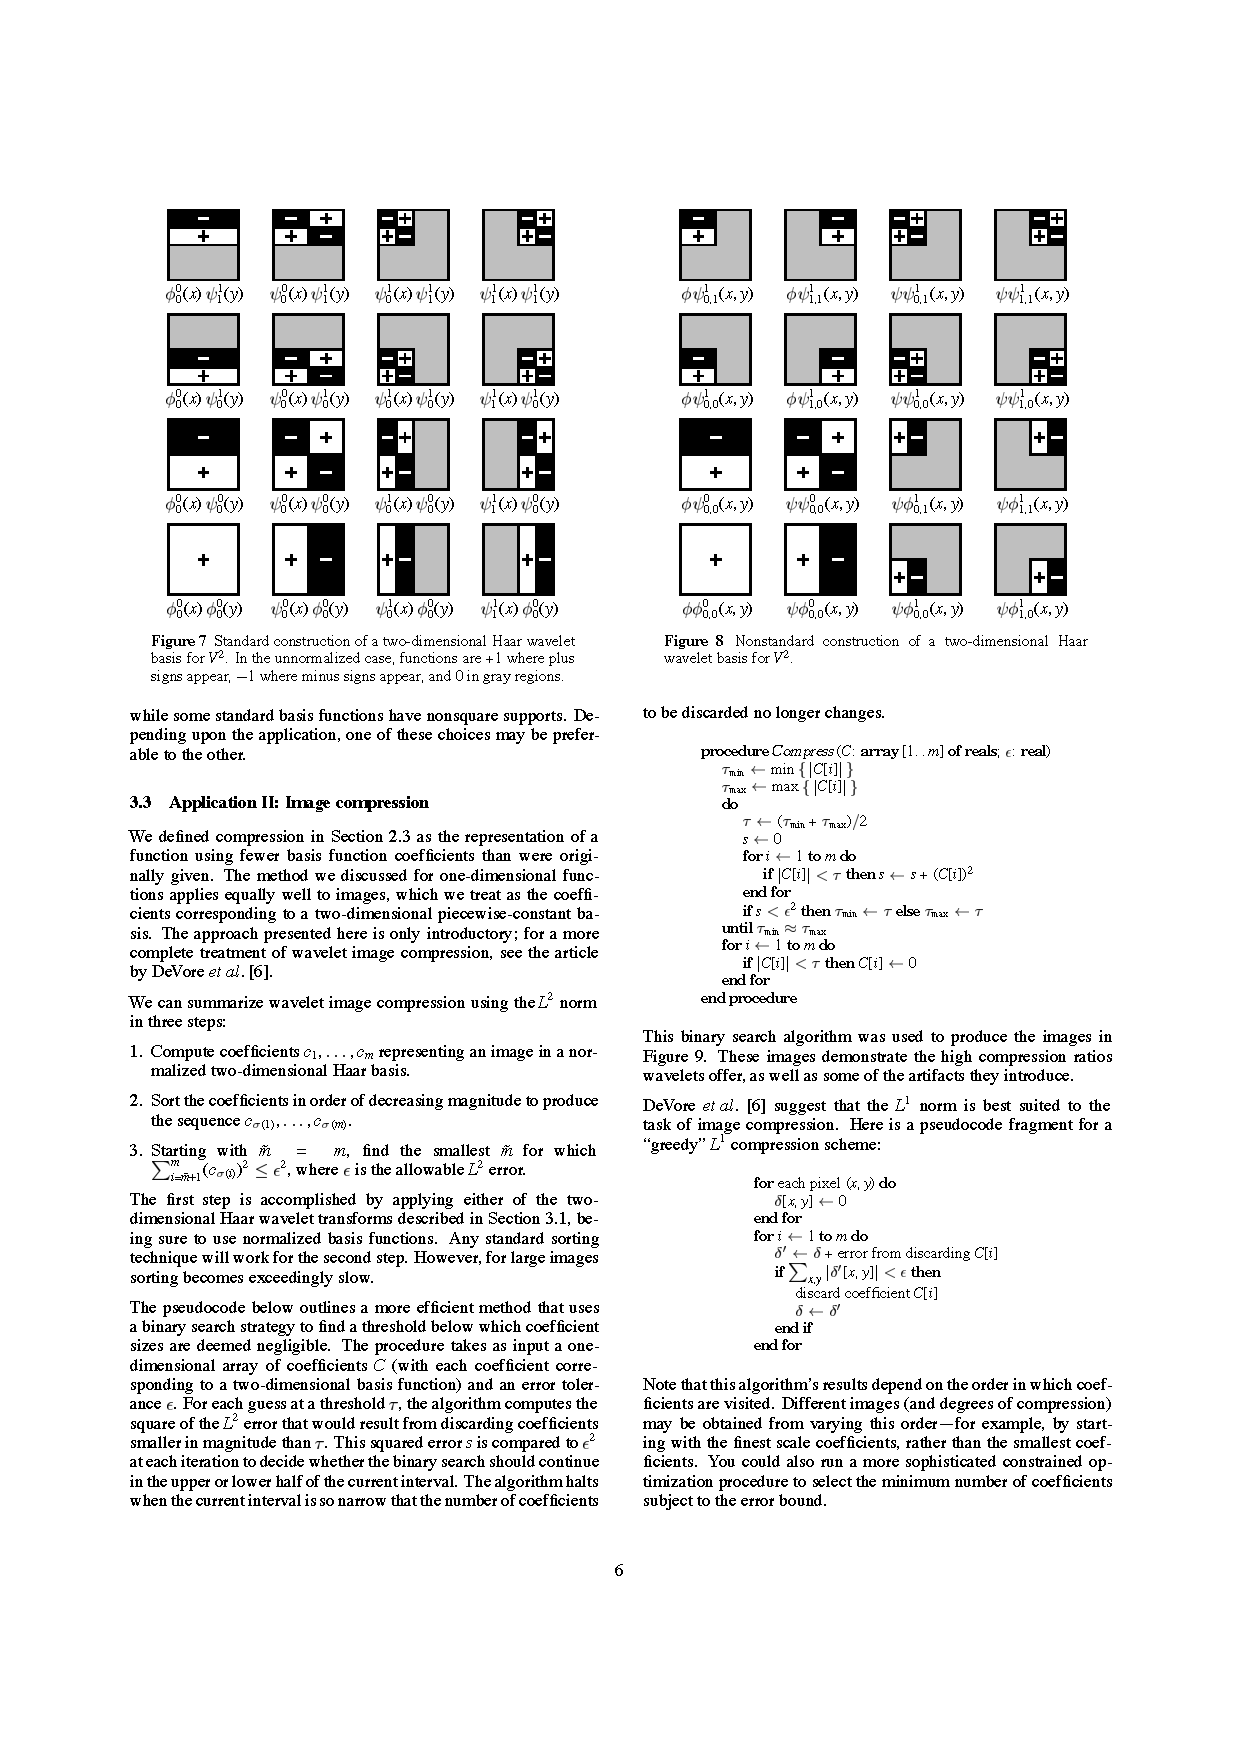
\includegraphics[trim=79 545 300 100, clip, width=0.45\textwidth]{2d_wavelets.pdf}
	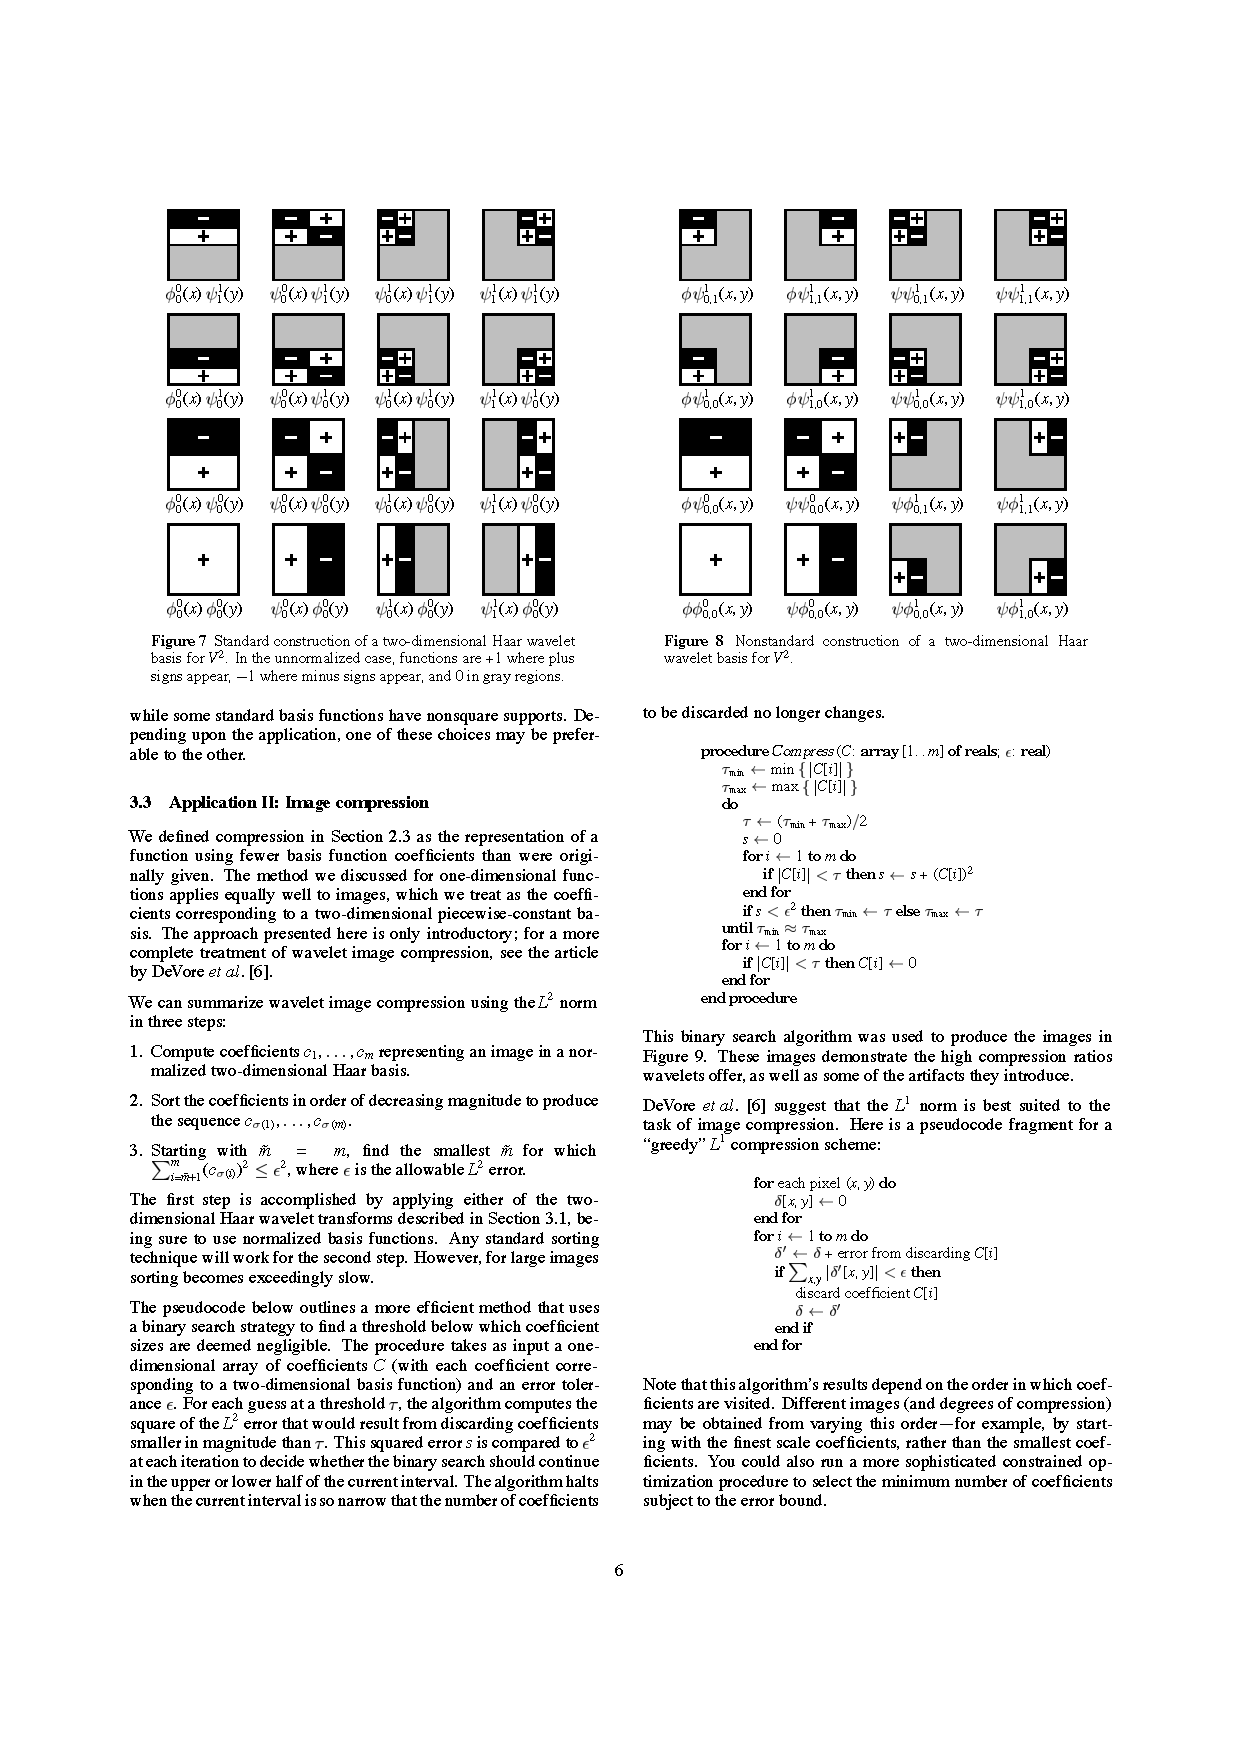
\includegraphics[trim=300 545 79 100, clip, width=0.45\textwidth]{2d_wavelets.pdf}
	\caption{2D Haar-Wavelets des $V_{2D}^3$: Standard-Konstruktion (links) und Nicht-Standard-Konstruktion (rechts)}
\end{figure}\\
Vorteil der Standard-Konstruktion ist die Möglichkeit nur 1D Wavelet-Transformation implementieren zu müssen, Nachteil ist ein etwas höherer Rechenaufwand. Außerdem unterscheiden sich beide Konstruktionen bezüglich der Form der Träger: Während die Nicht-Standard-Konstruktion ausschließlich Wavelets mit quadratischen Trägern hervorbringt, haben die Wavelets nach Standard-Konstruktion zu Teilen rechteckige Träger. Welche Methode besser geeignet ist, hängt somit vor allem von der Anwendung ab.
	
